\newpage
%\chapter{Results and discussion}

\section{Results and discussion}
In this section the results of the simulations will be presented and discussed. Two different variations of the LB solver were tested. One with the optimised values of the relaxation parameters~\cite{geier:parameter} and other with the relaxation parameters used as specified in ~\cite{geier:cumulant}. The results presented in this section are performed with the former variation of the LB solver  and the results of the latter variation will just be presented in the Appendix, as the choice of value one for all the parameters is the most stable choice but not accurate enough~\cite{geier:parameter}. Firstly, the results of the LB simulations carried out without any turbulence model will be presented and discussed. The result of the simulations with no-model will be termed as the \emph{under resolved DNS} (UDNS). Under resolved because the resolution is coarser compared to the reference mesh resolution and DNS because no additional modelling is done for turbulence. It will be followed by the discussion of the results from the LB-LES with the WALE model and will be compared with the UDNS and DNS results. Few general comments applicable for all the simulations are:

\begin{itemize}
\item The DNS results of~\cite{kim:moin:moser:87} , for $Re_\tau = 395$, will be used as a reference for the comparison. The quantities obtained from the DNS data will be referred to as the \emph{target} quantities.
\item The results shown here are plotted against the global coordinates, $y/\de$, and local coordinates,  $y^+$.  
\item All simulations have been performed using the single precision on GPGPUs. 
\item The normalised wall distance $y^+$ used in the profile plots is computed a posteriori for all the simulations.
%\item Since the channel flow is symmetric, the profiles have been plotted over the  
\end{itemize}

\subsection{UDNS results} \label{UDNS profiles}
To test the accuracy of the turbulent channel flow results from the LB solver, against the DNS data, these simulations have been performed. The physical quantities resulting from the simulations for all meshes are listed in the table (\ref{Global quantities}). The average friction velocity ($u_\tau$) and the $Re_\tau$ resulting from the computed $u_\tau$ are the important quantities. From now on $u_\tau$ represents the average friction velocity. The computed value of $u_\tau$ is under-predicted for all the simulations and so is the resulting $Re_\tau$, but the values approach the target $u_\tau$ with the increase in the mesh resolution. We know from the definition of $u_\tau$,that $u_\tau$ is proportional to the $\tau_w$. Thus, smaller values of the $u_\tau$ implies smaller values of $\tau_w$.  
%
\begin{table}[h!]
\begin{center}
\begin{tabular}{ p{3cm}|p{1.5cm}p{1.5cm}p{1.5cm}p{1.5cm}  } 
\hline
Physical quantity & Mesh1 & Mesh1\_5 & Mesh2 & Target \\
  \hline
  \multirow{1}{6em}{$u_\tau,\ m/s$}  & 0.0070 & 0.0074 & 0.0076 & 0.0079\\
  \hline
  \multirow{1}{6em}{$Re_\tau$} & 352 & 371 & 382 & 395\\
  \hline
  \multirow{1}{6em}{$U_c,\ m/s$} & 0.1565 & 0.1563 & 0.1557 & 0.1591\\
  \hline
\end{tabular}
\end{center}
\caption{Comparison of the resulting physical quantities}
\label{Global quantities}
\end{table}
%
\subsubsection{Mean velocity profile} \label{Mean velocity UDNS}

Mean velocity profiles presented here have been averaged in time and space. It is seen from the Fig. (\ref{Mean velocity global}) and Fig. (\ref{Mean velocity wall}), the mean velocity profiles for all the meshes over-predict the DNS data. As discussed in the section \ref{scaling} the viscous sublayer plays a dominant role on the flow characteristics as higher velocity gradients are present there. Since the viscous sublayer is under-resolved in the simulations, $u_\tau$ and eventually the $\tau_w$ is under-predicted and as a result we see the different flow characteristics obtained from the simulations i.e. over-predicting velocity profiles in comparison to the DNS data. It is clear that with the better resolution of the viscous sublayer, the correct flow characteristics will be obtained and it is apparent from the Fig. (\ref{Mean velocity global}) and Fig. (\ref{Mean velocity wall}) that with the mesh refinement, the velocity profiles approach closer to the DNS data. Velocity profile for mesh3 nearly collapses on to the DNS data. Thus a positive effect of mesh resolution is seen from the mean velocity profile plots. 
%
\begin{figure}[h]
    \centering
    \includegraphics[width=0.95\textwidth]{06_Resultsanddiscussion/figur/UDNS_2016/Profile_global_coords.png}
    \caption{Mean stream-wise velocity profile normalized by $u_\tau$, plotted in global coordinates}
    \label{Mean velocity global}
\end{figure}

\begin{figure}[t]
    \centering
    \includegraphics[width=0.95\textwidth]{06_Resultsanddiscussion/figur/UDNS_2016/Profile_wall_coords_theo_comp.png}
    \caption{Mean stream-wise  velocity profile normalized by $u_\tau$, plotted in wall coordinates (semi-log plot)}
    \label{Mean velocity wall}
\end{figure}

\subsubsection{Turbulence intensities} \label{Turbulence intensities UDNS}
Turbulence intensities is the term used for the root-mean-square (rms) profiles of the velocity fluctuations. The rms profiles shown in this section have been averaged in the following order: 
the time-averaged data set written out in every time-step is spatially averaged and these time and space averaged data sets are again time-averaged to have symmetric rms profiles. The Fig. \ref{Turbulence intensities} shows the rms velocity fluctuations plotted in the global coordinates. The rms profiles are symmetric about the half-channel height i.e. $y = \de$ and the symmetry of the profiles about $\de$ indicates the adequacy of the sampling taken for average ~\cite{kim:moin:moser:87}. Turbulence intensities normalised by $u_\tau$ are compared with different mesh resolutions and the DNS data\footnote{the DNS data for the velocity fluctuation profiles have been provided as variances ($\overline{{\up}^2}$) and not the rms ($\sqrt{\overline{{\up}^2}}$)values}. 
%
\begin{figure}[h!]
    \centering
    \includegraphics[width=0.6\textwidth]{06_Resultsanddiscussion/figur/UDNS_2016/Turbulence ontensities_Mesh2.jpg}
    \caption{Root-mean-square velocity fluctuations normalized by $u_\tau$ in global coordinates}
    \label{Turbulence intensities}
\end{figure}
%

Fig.(\ref{urms wall})-(\ref{wrms wall}) shows the comparison of the components of the rms profiles of the streamwise, wall-normal and spanwise velocity fluctuations, respectively, with the different mesh resolutions and the DNS data in wall coordinates. The profiles do not start from zero value, as only the fluid nodes are plotted. The general observation from all three velocity fluctuation profiles is that they converge to the DNS data with the increase in the mesh resolution. 

Mesh 2 and Mesh 3 accurately estimates the location of the peak values for all three velocity component profiles, respectively, compared to the DNS data. Mesh 3 for all the velocity component profiles predict the peak value fairly close to that of the DNS data. All three velocity component profiles for Mesh 3 are in fairly good agreement with the DNS data. 

The rms value of the streamwise profile increases from zero at the wall to some peak value in either buffer layer, $5<y^+< 30$, or in the log-law layer, $y^+ > 30\  till\  y/\de <0.3$ and then drops gradually towards the centre of the channel. The velocity profile for the wall-normal component develops slowly in comparison to the streamwise and the spanwise component profiles. The approximate location of the peak value for streamwise profile (DNS) is at $y^+ = 14$ \cite{kim:moin:moser:87} i.e. buffer layer. The location of peak value for the spanwise component (DNS) is at $y^+ = 40$ i.e. log-law region and the location for the wall-normal component (DNS)is at $y^+ = 70$ also in the log-law region, but towards the end of it. The resulting profiles of Mesh 3 for all components approximately shows the same locations for the peak values as that of the corresponding DNS data.
%%
%\begin{table}[h!]
%\begin{center}
%\begin{tabular}{ p{1cm}|p{1.5cm}p{1.5cm}p{1.5cm}p{1.5cm}  } 
%\hline
% & Mesh1 & Mesh2 & Mesh3 & DNS \\
%  \hline
%  \multirow{1}{6em}{$y^+$} & 17 & 15 & 14.93 & 14\\
%  \hline
%\end{tabular}
%\end{center}
%\caption{Peak values of the rms profiles of stream-wise velocity fluctuations}
%\label{Peak values}
%\end{table}
%%
%
\begin{figure}[h]
%\centering
\begin{minipage}[b]{0.5\textwidth}
\subfigure[Zoom near the wall]{
\includegraphics[width=6.7cm]{06_Resultsanddiscussion/figur/UDNS_2016/urms_global_coords.jpg}}
\end{minipage}
%
\begin{minipage}[b]{0.5\textwidth}
\subfigure[Outer region]{
\includegraphics[width=6.7cm]{06_Resultsanddiscussion/figur/UDNS_2016/urms_wall_coords.jpg}}
\end{minipage}
\caption{Channel flow at $Re_\tau=2000$}
\label{uv_balance}
\end{figure}


\begin{figure}[h!]
    \centering
    \includegraphics[width=0.6\textwidth]{06_Resultsanddiscussion/figur/UDNS_2016/urms_wall_coords.jpg}
    \caption{$u_{rms}$ normalized by $u_\tau$ in wall coordinates}
    \label{urms wall}
\end{figure}

\begin{figure}[h!]
    \centering
    \includegraphics[width=0.6\textwidth]{06_Resultsanddiscussion/figur/UDNS_2016/vrms_wall_coords.jpg}
    \caption{$v_{rms}$ normalized by $u_\tau$ in wall coordinates}
    \label{vrms wall}
\end{figure}

\begin{figure}[h!]
    \centering
    \includegraphics[width=0.6\textwidth]{06_Resultsanddiscussion/figur/UDNS_2016/wrms_wall_coords.jpg}
    \caption{$w_{rms}$ normalized by $u_\tau$ in wall coordinates}
    \label{wrms wall}
\end{figure}

\subsubsection{Turbulent shear stress}
Turbulent shear stress is also referred to as the co-variance of the Reynolds stress tensor i.e. $-\overline{\up\vp}$. This component is responsible for the turbulent diffusion of the momentum. It is also sometimes referred to as the resolved shear stress. 

Fig. (\ref{uvrms wall}) shows the turbulent shear stress profile normalised with the $u_\tau^2$ plotted in wall coordinates and compared against the DNS data and with the mesh resolutions.
\begin{figure}[h!]
    \centering
    \includegraphics[width=0.6\textwidth]{06_Resultsanddiscussion/figur/UDNS_2016/uv_rms_wall_coords.jpg}
    \caption{$uv_{rms}$ normalized by $u_\tau$ in wall coordinates}
    \label{uvrms wall}
\end{figure}

As seen from the Fig. (\ref{uvrms wall}) the increase in the mesh resolution results in the better agreement to the DNS data. Mesh 3 here shows a very good agreement to the DNS data and also it predicts the location of the peak value, $y^+ = 35$ fairly well.
\subsection{WALE model results}
In this section the results obtained from the combination of the LB flow solver with the WALE model (LES) performed on the relatively coarser mesh, in comparison to the resolution of the DNS data, will be presented. The main purpose is to access the accuracy with which the aforementioned combination reproduces the mean flow profiles and other turbulence statistics when compared to the DNS data. The computed physical quantities have been listed in the table \ref{Global quantities WALE} for all mesh resolutions. The same trend is seen for the physical quantities as mentioned in the section \ref{UDNS profiles}. The physical quantities approach closer to the respective target values with the increase in the mesh resolution. 
%
\begin{table}[h!]
\begin{center}
\begin{tabular}{ p{3cm}|p{1.5cm}p{1.5cm}p{1.5cm}p{1.5cm}  } 
\hline
Physical quantity & Mesh1 & Mesh2 & Mesh3 & Target \\
  \hline
  \multirow{1}{6em}{$u_\tau,\ m/s$}  & 0.0069 & 0.0073 & 0.0075 & 0.0079\\
  \hline
  \multirow{1}{6em}{$Re_\tau$} & 347 & 367 & 377 & 395\\
  \hline
  \multirow{1}{6em}{$U_c,\ m/s$} & 0.1562 & 0.1557 & 0.1547 & 0.1591\\
  \hline
\end{tabular}
\end{center}
\caption{Comparison of the computed physical quantities using WALE model}
\label{Global quantities WALE}
\end{table}
%
\subsubsection{Mean velocity profiles}
The mean velocity profiles, normalised with the $u_\tau$, presented here are averaged in time and space. Fig. (\ref{Mean profiles WALE}(a-b)) shows the mean velocity profiles plotted in the global and local coordinates. It is clear from the both the figures that with increase in the mesh resolution the velocity profiles approach closer to the DNS data. All profiles over-predict the DNS data, but the velocity profile for the mesh 3 is relatively in good agreement with the DNS data. The reason for the over-prediction is similar to that explained in section \ref{Mean velocity UDNS}.
%%% Mean veloity profiles %%%
\begin{figure}[h!]
%\centering
\begin{minipage}[b]{0.5\textwidth}
\subfigure[global coordinates]{
\includegraphics[width=6.7cm]{06_Resultsanddiscussion/figur/WALE/Profile_global_coords.png}}
\end{minipage}
%
\begin{minipage}[b]{0.5\textwidth}
\subfigure[wall coordinates]{
\includegraphics[width=6.7cm]{06_Resultsanddiscussion/figur/WALE/Profile_wall_coords_theo_comp.png}}
\end{minipage}
\caption{Mean velocity profile normalised with $u_\tau$}
\label{Mean profiles WALE}
\end{figure}
%%% End mean velociy profiles %%%%
\subsubsection{Turbulence intensities}
The rms profiles presented here are averaged in the same fashion as that of the section \ref{Turbulence intensities UDNS}. To show the adequacy of sampling taken for averaging the symmetric rms profiles, about the half-channel height $y  = \de$, of all three velocity fluctuations is shown in Fig. (\ref{Turbulence intensities WALE}). The comments made in the section \ref{Turbulence intensities UDNS} for the velocity profiles are also applicable here.
%
\begin{figure}[h!]
    \centering
    \includegraphics[width=0.6\textwidth]{06_Resultsanddiscussion/figur/WALE/Turbulence intensities_Mesh2.png}
    \caption{Root-mean-square velocity fluctuations normalized by $u_\tau$ in global coordinates}
    \label{Turbulence intensities WALE}
\end{figure}
%
The rms velocity profiles for all three components show a good agreement towards the DNS data as the mesh resolution increases. 
%
\begin{figure}[h!]
%\centering
\begin{minipage}[b]{0.5\textwidth}
\subfigure[global coordinates]{
\includegraphics[width=6.7cm]{06_Resultsanddiscussion/figur/WALE/urms_global_coords.png}}
\end{minipage}
%
\begin{minipage}[b]{0.5\textwidth}
\subfigure[local coordinates]{
\includegraphics[width=6.7cm]{06_Resultsanddiscussion/figur/WALE/urms_wall_coords.png}}
\end{minipage}
\caption{Rms profiles for the streamwise velocity fluctuation normalised by $u_\tau$}
\label{urms wale}
\end{figure}
%% End %%
%
\begin{figure}[h!]
%\centering
\begin{minipage}[b]{0.5\textwidth}
\subfigure[global coordinates]{
\includegraphics[width=6.7cm]{06_Resultsanddiscussion/figur/WALE/vrms_global_coords.png}}
\end{minipage}
%
\begin{minipage}[b]{0.5\textwidth}
\subfigure[local coordinates]{
\includegraphics[width=6.7cm]{06_Resultsanddiscussion/figur/WALE/vrms_wall_coords.png}}
\end{minipage}
\caption{Rms profiles for the wall-normal velocity fluctuation normalised by $u_\tau$}
\label{vrms wale}
\end{figure}
%% End %%
%
\begin{figure}[h!]
%\centering
\begin{minipage}[b]{0.5\textwidth}
\subfigure[global coordinates]{
\includegraphics[width=6.7cm]{06_Resultsanddiscussion/figur/WALE/wrms_global_coords.png}}
\end{minipage}
%
\begin{minipage}[b]{0.5\textwidth}
\subfigure[local coordinates]{
\includegraphics[width=6.7cm]{06_Resultsanddiscussion/figur/WALE/wrms_wall_coords.png}}
\end{minipage}
\caption{Rms profiles for the spanwise velocity fluctuation normalised by $u_\tau$}
\label{wrms wale}
\end{figure}
%% End %%
\subsubsection{Turbulent shear stress}
%
\begin{figure}[h!]
%\centering
\begin{minipage}[b]{0.5\textwidth}
\subfigure[global coordinates]{
\includegraphics[width=6.7cm]{06_Resultsanddiscussion/figur/WALE/uv_rms_global_coords.png}}
\end{minipage}
%
\begin{minipage}[b]{0.5\textwidth}
\subfigure[local coordinates]{
\includegraphics[width=6.7cm]{06_Resultsanddiscussion/figur/WALE/uv_rms_wall_coords.png}}
\end{minipage}
\caption{Turbulent shear stress profiles normalised by $u_\tau$}
\label{uvrms wale}
\end{figure}
%% End %%
%\subsection{Comparison UDNS and WALE}